% Poster created for ScienceDay2012
%
% @author Szilard VAJDA, Eugene Borovikov
% @date   2012 September 13

%\documentclass[landscape,a1,final]

% A1 size
\documentclass[landscape,a1]{a0poster}
% A0 size
%\documentclass[portrait,a0,final]{a0poster}
%\documentclass[landscape,a0,posterdraft]{a0poster}

%\renewcommand{\tiny}{\fontsize{12}{14}\selectfont}

%\renewcommand{\scriptsize}{\fontsize{14.4}{18}\selectfont}

%\renewcommand{\footnotesize}{\fontsize{17.28}{22}\selectfont}

%\renewcommand{\small}{\fontsize{20.74}{25}\selectfont}

%\renewcommand{\normalsize}{\fontsize{24.88}{30}\selectfont}

%\renewcommand{\large}{\fontsize{29.86}{37}\selectfont}

%\renewcommand{\Large}{\fontsize{35.83}{45}\selectfont}

%\renewcommand{\LARGE}{\fontsize{43}{54}\selectfont}

%\renewcommand{\huge}{\fontsize{51.6}{64}\selectfont}

%\renewcommand{\Huge}{\fontsize{61.92}{77}\selectfont}

%\newcommand{\veryHuge}{\fontsize{74.3}{93}\selectfont}

%\newcommand{\VeryHuge}{\fontsize{89.16}{112}\selectfont}

%\newcommand{\VERYHuge}{\fontsize{107}{134}\selectfont}
% As info the paper sizes:
%format  	paper size 	.ps bounding box size (portrait)
%A0 841 � 1189 mm	0 0 2383 3370
%A0b 841 x 
%A1 595 � 841 mm 0 0 1685 2383
%A2 420 � 595 mm 0 0 1192 1685
%A3 297 � 420 mm 0 0 842 1192
%A4 210 � 297 mm 0 0 595 842

\usepackage[american]{babel} 
\usepackage[paper=a0paper,landscape,noheadfoot,left=1cm,top=1cm,right=1cm,nohead,nofoot]{geometry}

%\usepackage[paper=a0paper,landscape,left=1cm,top=1cm,right=1cm,nohead]{geometry}

\usepackage{setspace} % stretch of baselineskip 
\usepackage{graphicx}
\usepackage{sectionbox}
\usepackage{enumitem}
\usepackage{color}
\usepackage[babel]{csquotes} % allow changing the quotation style
\usepackage[none]{hyphenat} % option 'none' to prevent any hyphenation throughout the document
\usepackage{pgfplots}
\usepackage{booktabs}
\usepackage{multicol}
\usepackage{textpos}


%% Changes in a0poster.cls:

%\ifanullb
%   \setlength{\paperwidth}{119cm}
%   \setlength{\paperheight}{88cm}
%   \setlength{\textwidth}{116cm}
%   \setlength{\textheight}{88cm}
%\else\ifanull
%        \setlength{\paperwidth}{118.82cm}
%        \setlength{\paperheight}{83.96cm}
%        \setlength{\textwidth}{117.82cm}
%        \setlength{\textheight}{82.96cm}
%     \else\ifaeins
%             \setlength{\paperwidth}{83.96cm}
%             \setlength{\paperheight}{59.4cm}
%             \setlength{\textwidth}{83.96cm}
%             \setlength{\textheight}{58.4cm}
%          \else\ifazwei
%                  \setlength{\paperwidth}{59.4cm}
%                  \setlength{\paperheight}{41.98cm}
%                  \setlength{\textwidth}{58.4cm}
%                  \setlength{\textheight}{40.98cm}
%               \else\ifadrei
%                       \setlength{\paperwidth}{41.98cm}
%                       \setlength{\paperheight}{29.7cm}
%                       \setlength{\textwidth}{40.98cm}
%                       \setlength{\textheight}{28.7cm}
%                    \else\relax
%                    \fi
%               \fi
%          \fi
%     \fi
%\fi
%\setlength{\topmargin}{-10.7 mm}  % -1in +1.47cm
%\setlength{\oddsidemargin}{-21.4 mm} % -1in +0.4cm

%\ifportrait
%   \newdimen\tausch
%   \setlength{\tausch}{\paperwidth}
%   \setlength{\paperwidth}{\paperheight}
%   \setlength{\paperheight}{\tausch}
%   \setlength{\tausch}{\textwidth}
%   \setlength{\textwidth}{\textheight}
%   \setlength{\textheight}{\tausch}
%\else\relax
%\fi


%% Additional commands:
%\makeatletter
%\renewcommand{\section}{\@startsection {section}{1}{\z@}%
%  {-3.5ex \@plus -1ex \@minus -.2ex}%
%  {2.3ex \@plus.2ex}%
%  {\reset@font\Large\bfseries\sffamily}}
%\renewcommand{\subsection}{\@startsection{subsection}{2}{\z@}%
%  {-3.25ex\@plus -1ex \@minus -.2ex}%
%  {1.5ex \@plus .2ex}%
%  {\reset@font\large\bfseries\sffamily}}
%\makeatother

%%%%%%%%%%%%%%%%%%%%%%%%%%%%%%%%%%%%%%%%%%%%%%%%%%%%
%%%               Hintergrund                    %%%
%%%%%%%%%%%%%%%%%%%%%%%%%%%%%%%%%%%%%%%%%%%%%%%%%%%%
\newcommand{\background}[3]{\newrgbcolor{cgradbegin}{#1}
  \newrgbcolor{cgradend}{#2} 
  \psframe[fillstyle=gradient,gradend=cgradend,
  gradbegin=cgradbegin,gradmidpoint=#3](0.,0.)(1.\textwidth,-1.\textheight)}

%%%%%%%%%%%%%%%%%%%%%%%%%%%%%%%%%%%%%%%%%%%%%%%%%%%%
%%%                Header                        %%%
%%%%%%%%%%%%%%%%%%%%%%%%%%%%%%%%%%%%%%%%%%%%%%%%%%%%
%\newenvironment{header}[1][1. 1. 1.] {
%    \vspace{2em}
%
%    \begin{center}
%    \newrgbcolor{hcolor}{#1}
%    \begin{lrbox}{\dummybox} 
%    \begin{minipage}[t]{.9\textwidth}
% }
% {  \end{minipage} \end{lrbox}
%      \raisebox{-\depth}{\hspace{.5in}\hspace{-4mm}
%       \psshadowbox[fillstyle=solid,fillcolor=hcolor,framesep=8mm]
%    {\usebox{\dummybox}}} \end{center}
%     \vspace{2em}
% }
\newenvironment{header}[1][1. 1. 1.] {} {}


%%%%%%%%%%%%%%%%%%%%%%%%%%%%%%%%%%%%%%%%%%%%%%%%%%%%
%%%                Header no shadow              %%%
%%%%%%%%%%%%%%%%%%%%%%%%%%%%%%%%%%%%%%%%%%%%%%%%%%%%
\newenvironment{headerns}[1][1. 1. 1.] {
    \vspace{2em}

    \begin{center}
    \newrgbcolor{hcolor}{#1}
    \begin{lrbox}{\dummybox} 
    \begin{minipage}[t]{.9\textwidth}
 }
 {  \end{minipage} \end{lrbox}
      \raisebox{-\depth}{\hspace{.5in}\hspace{-4mm}
       \psshadowbox[fillstyle=solid,fillcolor=hcolor,framesep=8mm,shadowsize=0pt]
    {\usebox{\dummybox}}} \end{center}
     \vspace{2em}
 }

%%%%%%%%%%%%%%%%%%%%%%%%%%%%%%%%%%%%%%%%%%%%%%%%%%%%
%%%                Poster                        %%%
%%%%%%%%%%%%%%%%%%%%%%%%%%%%%%%%%%%%%%%%%%%%%%%%%%%%
\newsavebox{\dummybox}
\newsavebox{\spalten}

%\newenvironment{poster} {
%   \vfill \begin{minipage}{\textwidth}  }
%  {\end{minipage} \vfill}
\newenvironment{poster}{
  \begin{center}
  \begin{minipage}[c]{0.975\textwidth}
 }{
  \end{minipage} 
  \end{center}
}

%%%%%%%%%%%%%%%%%%%%%%%%%%%%%%%%%%%%%%%%%%%%%%%%%%%%
%%%                pcolumn                       %%%
%%%%%%%%%%%%%%%%%%%%%%%%%%%%%%%%%%%%%%%%%%%%%%%%%%%%
%\newcommand{\columnfrac}{.3}
%\newenvironment{pcolumn}{%
%  \hfill\begin{minipage}[t]{\columnfrac\textwidth}}{\end{minipage}\hfill%
%}
\newenvironment{pcolumn}[1]{
  \begin{minipage}{#1\textwidth}
  \begin{center}
}{
  \end{center}
  \end{minipage}
}

%%%%%%%%%%%%%%%%%%%%%%%%%%%%%%%%%%%%%%%%%%%%%%%%%%%%
%%%                pbox                          %%%
%%%%%%%%%%%%%%%%%%%%%%%%%%%%%%%%%%%%%%%%%%%%%%%%%%%%
%\newenvironment{pbox}[1][1. 1. 1.] {
%   \newrgbcolor{bcolor}{#1}
%  \begin{lrbox}{\dummybox}%
%    \begin{minipage}{0.96\linewidth}}%
%    {\end{minipage}
%  \end{lrbox}
%  \raisebox{-\depth}{\hspace{-.5em} 
%   \psshadowbox[fillstyle=solid,fillcolor=bcolor,framesep=1em]{\usebox{\dummybox}}} \vspace{2em} \vfill}
\newenvironment{pbox}[1][1. 1. 1.] {
   \newrgbcolor{bcolor}{#1}
  \begin{lrbox}{\dummybox}%
    \begin{minipage}{0.96\linewidth}}%
    {\end{minipage}
  \end{lrbox}
  \raisebox{-\depth}{\hspace{-.5em} 
   \psshadowbox[fillstyle=solid,fillcolor=bcolor,framesep=1em]{\usebox{\dummybox}}} \vspace{2em} \vfill}

%%%%%%%%%%%%%%%%%%%%%%%%%%%%%%%%%%%%%%%%%%%%%%%%%%%%
%%%                pbox   no shadow              %%%
%%%%%%%%%%%%%%%%%%%%%%%%%%%%%%%%%%%%%%%%%%%%%%%%%%%%
\newenvironment{pboxns}[1][1. 1. 1.] {
   \newrgbcolor{bcolor}{#1}
  \begin{lrbox}{\dummybox}%
    \begin{minipage}{0.96\linewidth}}%
    {\end{minipage}
  \end{lrbox}
  \raisebox{-\depth}{\hspace{-.5em} 
   \psshadowbox[fillstyle=solid,fillcolor=bcolor,framesep=1em,shadowsize=0pt]{\usebox{\dummybox}}} \vspace{2em} \vfill}




\definecolor{seprulecolor}{gray}{0.95}

%\definecolor{tugreen1}{rgb}{.52,.72,.10}	% 84b819
\definecolor{tugreen1}{rgb}{.105,.239,.478}	% 84b819
\newcommand{\tugreen}[1]{{\color{tugreen1}{#1}}}

\definecolor{sectboxfillcol}{rgb}{1,1,1}
\definecolor{sectboxrulecol}{rgb}{.105,.239,.478}
\definecolor{shadowcolor}{gray}{0.30}
\newcommand{\shadowcolor}{shadowcolor}
\setlength{\shadowsize}{4pt}

%\newcommand{\Content}{\fontsize{36}{39}\selectfont} % f�r a0
%\newcommand{\Heading}{\fontsize{60}{75}\selectfont}
%\newcommand{\Authors}{\fontsize{43}{54}\selectfont} 
%%\newcommand{\Authors}{\Content} 
%%\newcommand{\Institutes}{\fontsize{43}{54}\selectfont} 
%%\newcommand{\Subtitle}{\fontsize{45}{58}\selectfont}
%\newcommand{\Institutes}{\Content} 
%\newcommand{\Caption}{\fontsize{30}{33}\selectfont}
%\newcommand{\Tabular}{\fontsize{24}{26}\selectfont} % f�r a0
%\newcommand{\Titlesize}{\fontsize{45}{58}\selectfont}
%\newcommand{\Subtitlesize}{\fontsize{36}{39}\selectfont}

\newcommand{\Content}{\normalsize} % f�r a0
\newcommand{\Heading}{\fontsize{60}{75}\selectfont}
\newcommand{\Authors}{\LARGE} 
%\newcommand{\Authors}{\Content} 
%\newcommand{\Institutes}{\fontsize{43}{54}\selectfont} 
%\newcommand{\Subtitle}{\fontsize{45}{58}\selectfont}
\newcommand{\Institutes}{\Large} 
\newcommand{\Caption}{\fontsize{30}{33}\selectfont}
\newcommand{\Tabular}{\fontsize{24}{26}\selectfont} % f�r a0
\newcommand{\Titlesize}{\large}
\newcommand{\Subtitlesize}{\normalsize}

\newcommand{\textsubscript}[1]{$_\mathrm{#1}$}

% make everything ultra-compact by eliminating most spaces ...
\setlength{\parskip}{0pt}
\setlength{\parsep}{0pt}
\setlength{\headsep}{0pt}
\setlength{\topskip}{0pt}
\setlength{\topmargin}{0pt}
\setlength{\topsep}{0pt}
\setlength{\partopsep}{0pt}
% ... and readjust some exceptions
%\parskip 5.0ex
\parskip 2.5ex


\renewcommand{\rmdefault}{phv}
\renewcommand{\familydefault}{\sfdefault}

%%%%%%%%%%%%%%%%%%%%%%%%%%%%%%%%%%%%%%%%%%%
% Definition of some variables and colors
%\renewcommand{\rho}{\varrho}
%\renewcommand{\phi}{\varphi}
\setlength{\columnsep}{1.5cm}
\setlength{\columnseprule}{2mm}
\setlength{\parindent}{0.0cm}

\renewcommand{\columnseprulecolor}{\color{seprulecolor}}

\setdescription{font=\sffamily\bfseries}
%\setitemize[1]{label={\Caption$\bullet$}}
%\setitemize[2]{label={\Caption$\bullet$}}
%\setitemize[3]{label={\Caption$\bullet$}}
%\setitemize[1]{label={\Content$\bullet$}}
%\setitemize[2]{label={\Content$\bullet$}}
%\setitemize[3]{label={\Content$\bullet$}}
\setitemize[1]{label={\Content\textbullet}}
\setitemize[2]{label={\Content\textbullet}}
\setitemize[3]{label={\Content\textbullet}}
%\setitemize[1]{label=$\circ$}
%\setitemize[2]{label=$\circ$}
%\setitemize[3]{label=$\circ$}

\newcommand{\itemarrow}{$\Rightarrow$\hspace{-0.2cm}}

% for labeled itemize environments
%\newcommand\litem[1]{\item{\bfseries #1,\enspace}}
\newcommand\litem[1]{\item{\sffamily\bfseries #1\enspace}}

% to (manually) control the layout of items (especially the spacing) in descriptions
%\newcommand\ditem[2]{\item[1]{\enspace#1}}
\newcommand\ditem[1][~]{\item[#1\enspace]}

%\newenvironment{descreplace}{\begin{itemize}[align=right,leftmargin=6cm,font=\sffamily\bfseries]}{\end{itemize}}
\newlength\descreplacemargin
\setlength{\descreplacemargin}{5.5cm}
\newenvironment{descreplace}[1][\descreplacemargin]{%
	\begin{itemize}[align=right,leftmargin=#1,font=\sffamily\bfseries]%
}{%
	\end{itemize}
}

\shadowsectionbox
\shadowsubsectionbox

\newenvironment{xsectionbox}[3][\columnwidth]{% default width of minipage is \columnwidth
\setlength{\fboxsep}{0.5\fboxrule}% ensures colorbox is filled up to boundary of sectionbox 
\begin{lrbox}{\sectsavebox} % open lrbox and save in \sectsavebox
\begin{minipage}{#1-2\colboxsep-3\fboxrule}
\color{sectboxtextcol}%
%\ifthenelse{\equal{#2}{}}{}{\section{#2}}%  only produce section if mandatory parameter not empty
%\ifthenelse{\equal{#3}{}}{}{#3}%  only produce section if mandatory parameter not empty
\ifthenelse{\equal{#2}{}}{}{{\vspace*{0.2cm}\noindent\hspace*{0.2cm}{\bf\Titlesize #2}\newline}}%  only produce title if mandatory parameter not empty
\ifthenelse{\equal{#3}{}}{%
\ifthenelse{\equal{#2}{}}{}{\vspace{-0.75cm}}%
}{%
{\noindent\hspace*{0.2cm}{\bf\Titlesize #3}\newline}\vspace{-0.75cm}%
}%  only produce subtitle if mandatory parameter not empty
%\vspace{-0.75cm}
}{%
%\vspace*{0.1cm}
\end{minipage}
\end{lrbox}                                  % close lrbox
  \color{sectboxrulecol}                     % sets color of boundary
  \noindent
  \makesectionbox{\setlength{\fboxsep}{\colboxsep}\colorbox{sectboxfillcol}{\usebox{\sectsavebox}}}               
  \\[\sectboxskip]
}

\newenvironment{xpsectionbox}[3][\columnwidth]{% default width of minipage is \columnwidth
\setlength{\fboxsep}{0.5\fboxrule}% ensures colorbox is filled up to boundary of sectionbox 
\begin{lrbox}{\sectsavebox} % open lrbox and save in \sectsavebox
\begin{minipage}{#1-2\colboxsep-3\fboxrule}
\color{sectboxtextcol}%
%\ifthenelse{\equal{#2}{}}{}{\section{#2}}%  only produce section if mandatory parameter not empty
%\ifthenelse{\equal{#3}{}}{}{#3}%  only produce section if mandatory parameter not empty
\ifthenelse{\equal{#2}{}}{}{{\vspace*{0.2cm}\noindent\hspace*{0.2cm}{\bf\Titlesize #2}\newline}}%  only produce title if mandatory parameter not empty
\ifthenelse{\equal{#3}{}}{}{{\noindent\hspace*{0.2cm}{\bf\Titlesize #3}\newline}}%  only produce subtitle if mandatory parameter not empty

\begin{minipage}{1.0\linewidth}
}{%
\end{minipage}
%\vspace*{0.1cm}
\end{minipage}
\end{lrbox}                                  % close lrbox
  \color{sectboxrulecol}                     % sets color of boundary
  \noindent
  \makesectionbox{\setlength{\fboxsep}{\colboxsep}\colorbox{sectboxfillcol}{\usebox{\sectsavebox}}}               
  \\[\sectboxskip]
}

\newcommand{\xpartbox}[1]{%
	%\renewcommand{\sectboxfillcol}{\tugreen}
	\definecolor{sectboxfillcol}{rgb}{.105,.239,.478}
	\begin{xsectionbox}{}{}
		\begin{center}
		{\Large \bf \color{white} #1}	
		\end{center}
	\end{xsectionbox}
	\definecolor{sectboxfillcol}{rgb}{1.,1.,1.}
}

\newlength{\mytablespace}
\setlength{\mytablespace}{0.25cm}
\newenvironment{mytable}[1][\mytablespace]{%
	\newcommand*{\fuckthatlatexcrap}{#1}
	\nobreak\vspace*{\fuckthatlatexcrap}
	\begin{center}
}{%
	\end{center}
	\nobreak\vspace*{\fuckthatlatexcrap}
}

\newcommand{\opt}{\operatornamewithlimits{opt}}
\newcommand{\sgn}{\operatornamewithlimits{sgn}}
\newcommand{\argmax}{\operatornamewithlimits{argmax}}
\def\bigdot{\ensuremath{\bullet}}        % dicker schwarzer Punkt
\def\cel{\ensuremath{^{\circ}C}}         % Grad Celsius
\def\grad{\ensuremath{^\circ}}           % Grad
\def\degree{\ensuremath{^\circ}}         % Grad

%%%%%%%%%%%%%%%%%%%%%%%%%%%%%%%%%%%%%%%%%%%%%%%%%%%%%%%%%%%%%%%%%%%%%%
%%% Begin of Document
%%%%%%%%%%%%%%%%%%%%%%%%%%%%%%%%%%%%%%%%%%%%%%%%%%%%%%%%%%%%%%%%%%%%%%

\begin{document}

\begin{header}
%%%
% DSS in the corner (for ICMI doctoral spotlight session)
%%%
% A0 841 � 1189 mm	0 0 2383 3370
% %A1 595 � 841 mm 0 0 1685 2383
%\begin{textblock*}{2.5cm}(1095mm,795mm)
%\begin{textblock*}{2.5cm}(1095mm,805mm)
%\begin{textblock*}{2.5cm}(841mm,595mm)
\begin{textblock*}{2.5cm}(1095mm,785mm)
	\begin{minipage}[b]{7.5cm}
		\begin{flushright}
			{ \bf \fontsize{60}{75}\selectfont\noindent CEB\noindent }
			%{ \bf \Large DSS }
		\end{flushright}
	\end{minipage}
\end{textblock*}
%\vspace{-2.5cm} % -- subtract the allocated textblock height

%%%
% DSS in the corner (for ICMI doctoral spotlight session)
%%%
% A0 841 � 1189 mm	0 0 2383 3370
%\begin{textblock*}{2.5cm}(10mm,785mm)
%\begin{textblock*}{2.5cm}(10mm,795mm)
%\begin{textblock*}{2.5cm}(10mm,805mm)
%\begin{textblock*}{2.5cm}(10mm,585mm)
\begin{textblock*}{2.5cm}(10mm,785mm)
	\begin{minipage}[b]{14.5cm}
		\begin{flushleft}
			{ \bf \footnotesize\selectfont {\noindent $26^{th}$ Annual NIH Research Festival\\ \noindent Bethesda, MD, USA, 2012 October 9-12\\[0mm]} }
		\end{flushleft}
	\end{minipage}
\end{textblock*}
\vspace*{-2.5cm} % -- subtract the allocated textblock height

%%%
% Logos
%%%
\begin{minipage}[t]{0.24\textwidth}
  \par\vspace*{-2.5em}
  %\vspace*{-3em}
  %\hspace*{-40cm}
	\begin{flushleft}
		%\includegraphics[height=4cm]{images/tud_logo_rgb.jpg}%
		
\includegraphics[height=6cm]{images/nlm_logo.jpg}
	\end{flushleft}
\end{minipage}
\hfill
\begin{minipage}[t]{0.5\textwidth}
  \begin{center}
  

    { \bf \veryHuge {FaceMatch: Visual Search for Pictures of Missing Persons During a Disaster Event} }
  \end{center}
\end{minipage}
\hfill
\begin{minipage}[t]{0.24\textwidth}
	\par\vspace*{-2.5em}
	%\vspace*{-2.5em}
	%\hspace*{-4cm}
	\begin{flushright}
 		%\includegraphics[height=4cm]{images/tu_inf_logo.png}
 		%\includegraphics[height=5cm]{images/fbi_logo_de.pdf}%
 		
\includegraphics[height=6cm]{images/nih_logo.jpg}
	\end{flushright}
\end{minipage}

%%%
% Titel
%%%
\vspace*{-2cm}
\begin{center}
	\begin{minipage}[t]{0.95\textwidth}
		\begin{center}
			%{ \bf \Heading \textsc{Multi-Modal and Multi-Camera Attention \\ in Smart Environments\\[10mm]}}
			\vspace{2cm}
			{\Authors Eugene Borovikov, Szil\'{a}rd Vajda, Girish Lingappa, Sameer Antani, Michael Gill, George R. Thoma}
			\vspace{1cm}
			{	\Institutes \centerline{ Communications Engineering Branch,  Lister Hill National Center for Biomedical Communications, U.S. National Library of Medicine, Bethesda, MD, 20894, USA}}
		\end{center}
	\end{minipage}
\end{center}

\end{header}

%Szilard
\vspace*{0.5cm}
%\vspace*{0.25cm}

\begin{poster}

%%% Begin of Multicols-Enviroment
\begin{multicols}{3}

\xpartbox{Abstract}

\begin{xpsectionbox}{}{}

\emph{\color{blue} NLM’s People Locator system allows the posting of photos and simple metadata (name, age, location) for persons missing (or found) in the wake of a disaster. To extend the current text-based search method to a visual search for people's faces, we developed FaceMatch, a system to match faces in a query image to those in the stored photos.
	Face matching is a two-stage process: faces in photos sent as queries are first localized using an improved Viola-Jones face detector, and then image features (SIFT, SURF, ORB and HAAR) are extracted, combined and matched against an index of features extracted from the stored photos. 
Face matching is challenging because of the lack of training data, low-resolution photos, wide variability in lighting, facial expression, head pose, ethnicity, occlusions and deformed faces due to injury.
Ongoing research, using images collected from the 2010 earthquake in Haiti and Labeled Faces in the Wild dataset, includes exploring more discriminating features, modeling skin color for more accurate face localization, a Haar wavelet-based technique to eliminate near-duplicate photos, and image normalization. FaceMatch speed and accuracy performance results are presented.}


\end{xpsectionbox}

\begin{xpsectionbox}{Challenges}{}

\begin{minipage}{0.45\linewidth}
\begin{itemize}
	 \item size of the database is about $15$K images
	 \item pictures may contain $0$, $1$, $2$, $\ldots N$ faces
	 \item face-like objects (cats and dogs faces)
	 \item query/database images may be of suboptimal quality due to
	 \item partially occluded or damaged faces
	\item presence of duplicates and near-duplicates
	\item inconsistency due to facial hair, glasses, jewelry, aging

\end{itemize}
\end{minipage}
\begin{minipage}{0.55\linewidth}
\begin{center}

			\vspace{-1cm}
			
			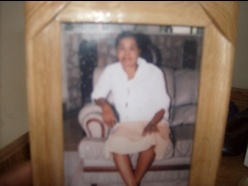
\includegraphics[height=0.22\linewidth]{images/PL_low_quality}
			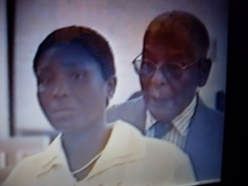
\includegraphics[height=0.22\linewidth]{images/HEPL_low_quality}
			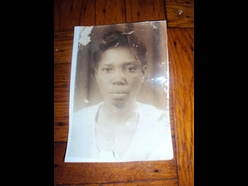
\includegraphics[height=0.22\linewidth]{images/HEPL_picture_photo}

			\vspace{0.2cm}			
			
			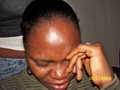
\includegraphics[height=0.22\linewidth]{images/HEPL_occlusion}
			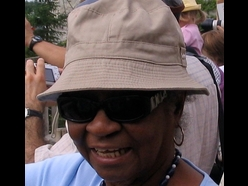
\includegraphics[height=0.22\linewidth]{images/HEPL_sunglasses_hat}
			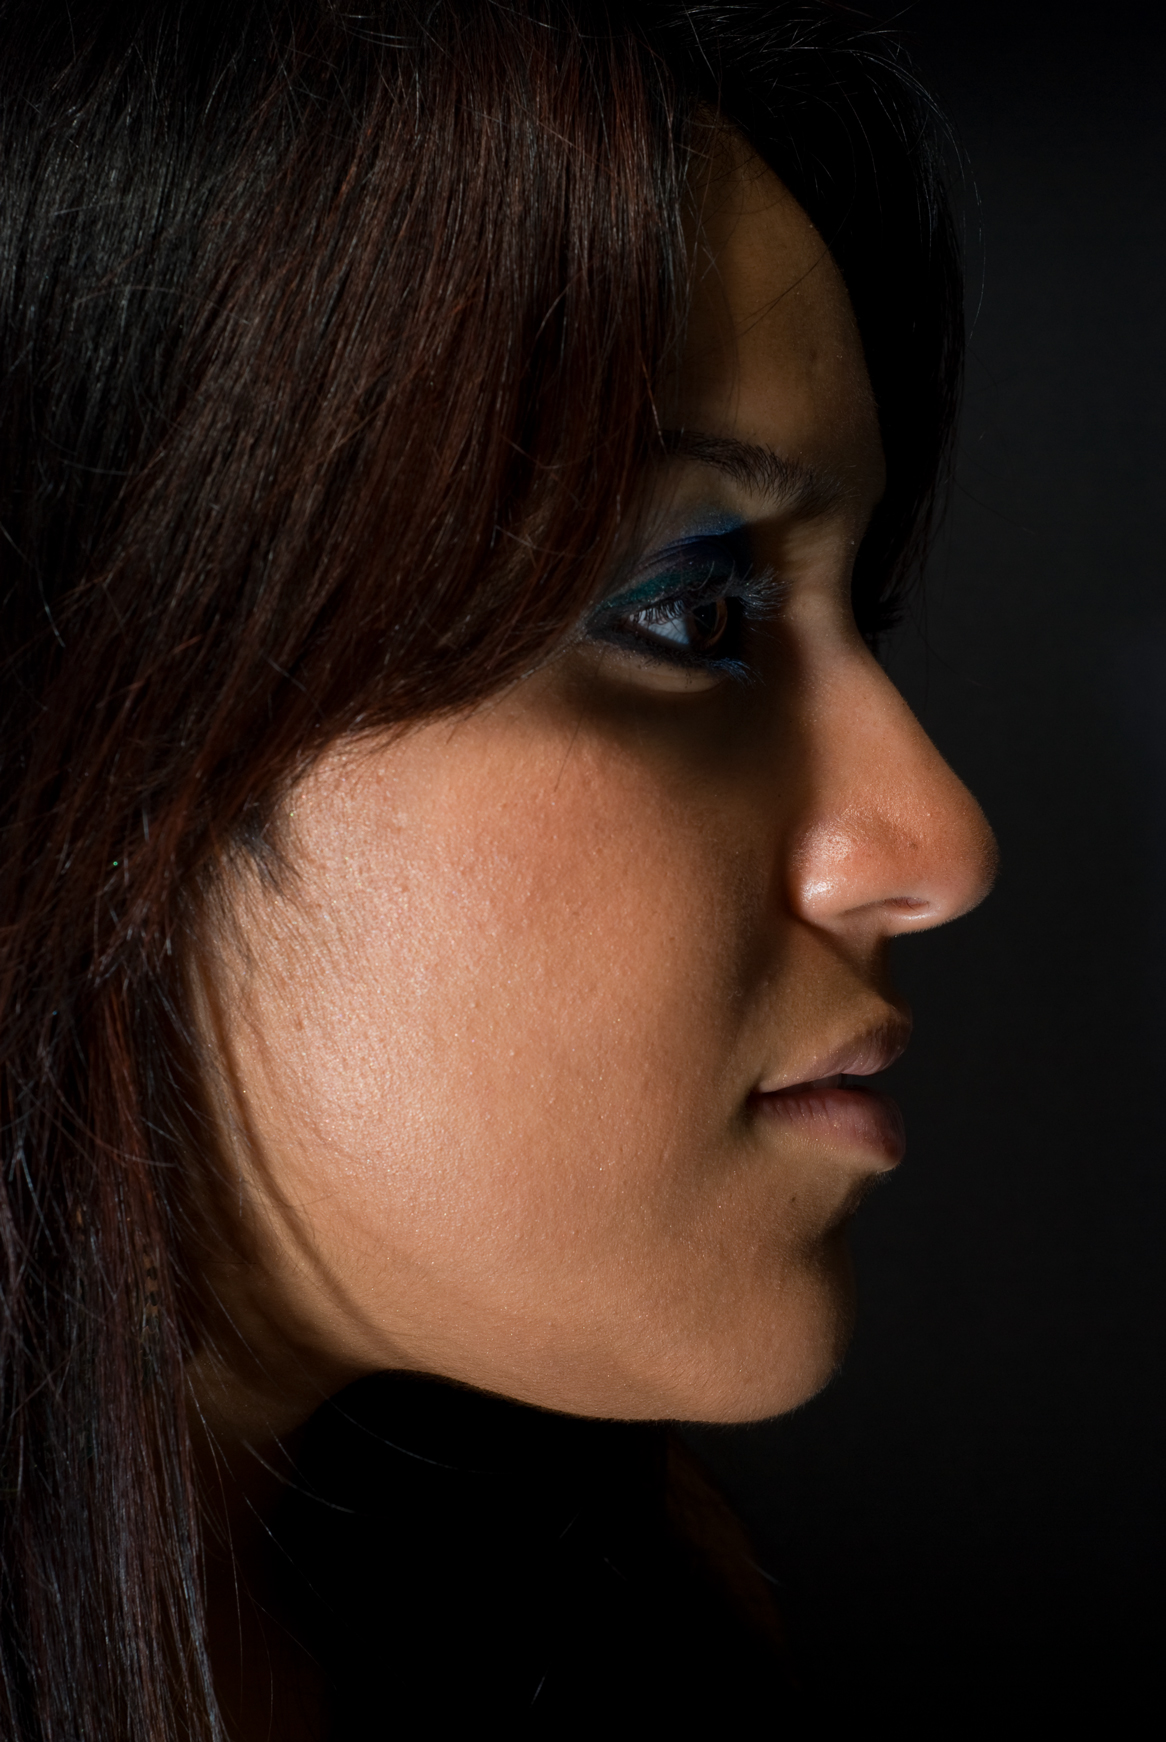
\includegraphics[height=0.22\linewidth]{images/AFLW_profile_dark}
\end{center}
\end{minipage}

\end{xpsectionbox}



\xpartbox{Application/Software}

\begin{xpsectionbox}{}{}

\begin{minipage}{0.4\linewidth}
\begin{itemize}
	\item important/helpful in disaster scenarios
	\item complementarity between text and images
	\item web interface
		\begin{itemize}
			\item intuitive
			\item accessibility from remote places
		\end{itemize}
\end{itemize}
\end{minipage}
\begin{minipage}{0.6\linewidth}
\begin{center}
	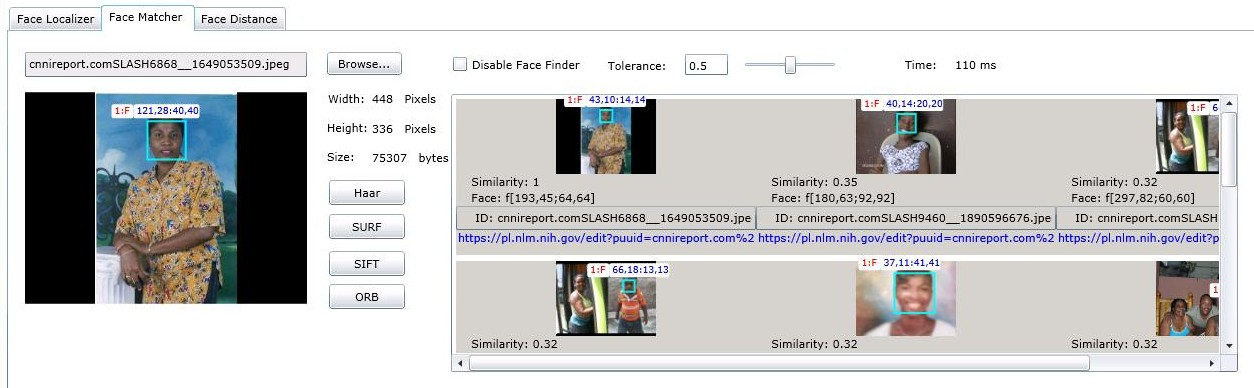
\includegraphics[height=0.5\linewidth]{images/web_interface}
\end{center}
\end{minipage}

%\begin{minipage}{0.4\linewidth}
%
%\begin{itemize}
%	  \item low-level image features (Haar, LBP, etc.)
%	  \item high-level facial landmarks (eye(s), nose, mouth, ear(s), chin, etc.)
%	  \item skin color
%\end{itemize}
%\end{minipage}
%\begin{minipage}{0.6\linewidth}
%
%\begin{center}
%%			%\hspace{-5cm}
%%			\vspace{-1cm}
%			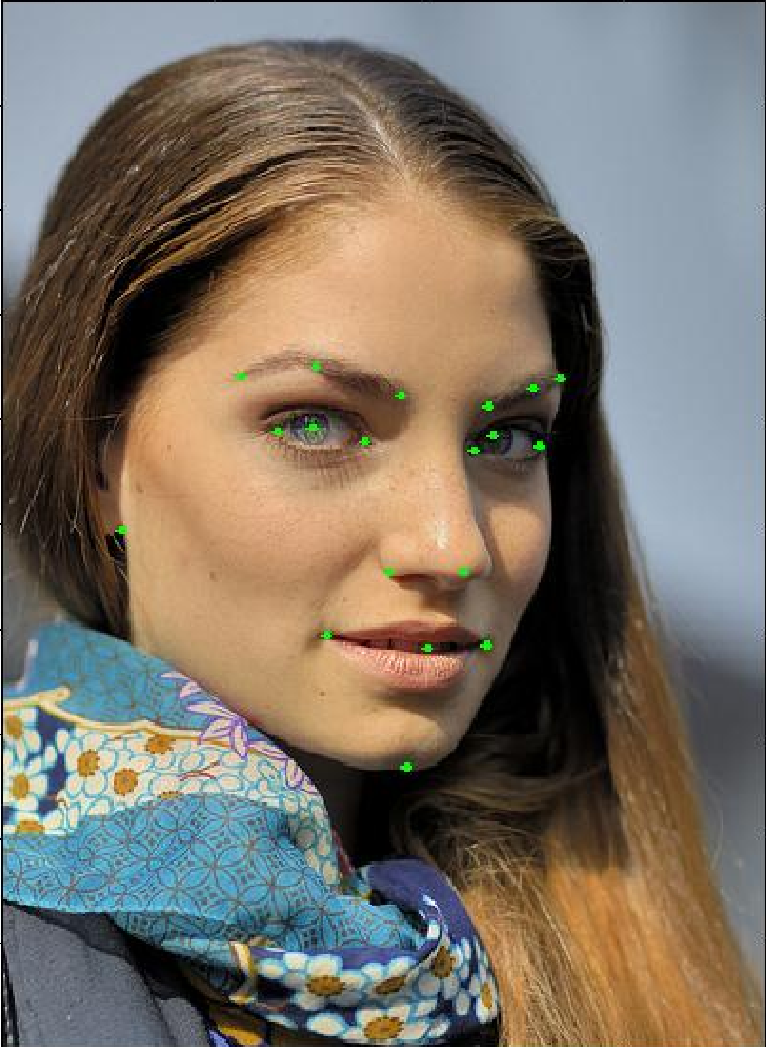
\includegraphics[height=0.25\linewidth]{images/facial_landmarks}
%			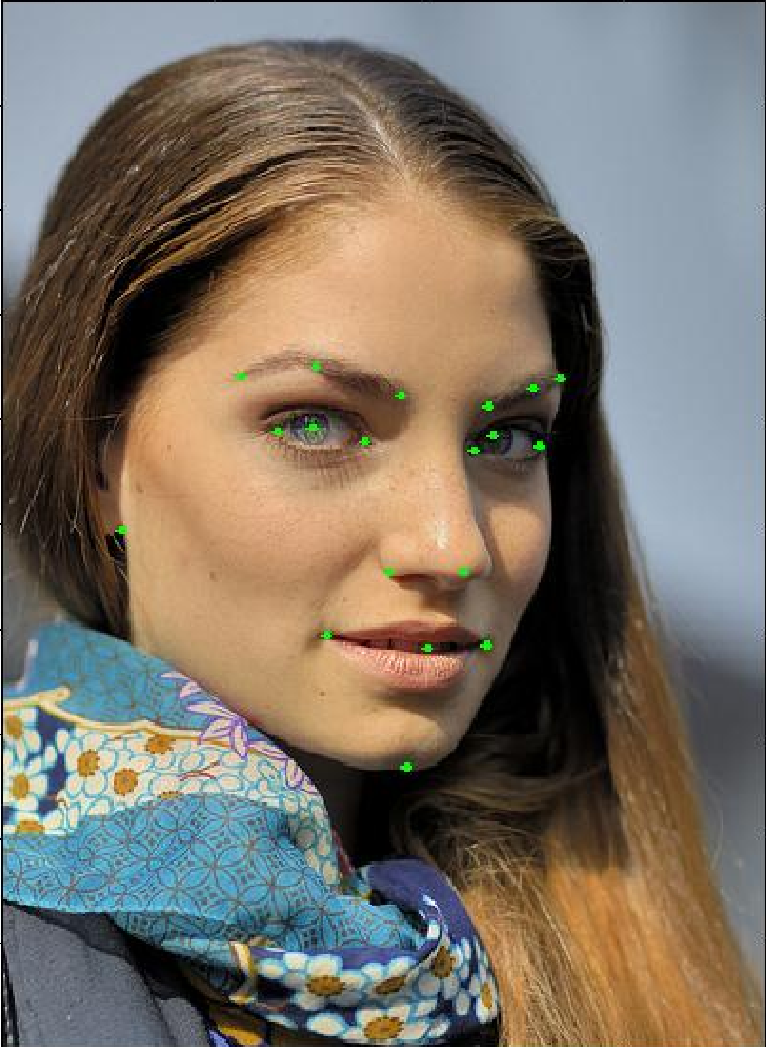
\includegraphics[height=0.25\linewidth]{images/facial_landmarks}
%\end{center}
%
%\end{minipage}
%\end{xpsectionbox}
%
%\begin{xpsectionbox}{Challenges}{}
%
%\begin{minipage}{0.4\linewidth}
%\begin{itemize}
%	  \item low-quality images
%	  \item various lighting conditions
%	  \item frontal vs. profile faces
%	  \item various skin colors
%	  \item occlusions, facial hair, spectacles, hat, etc.
%\end{itemize}
%\end{minipage}
%\begin{minipage}{0.6\linewidth}
%\begin{center}
%			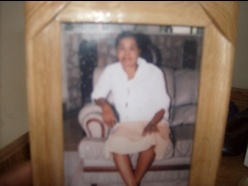
\includegraphics[height=0.25\linewidth]{images/PL_low_quality}
%			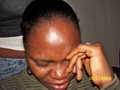
\includegraphics[height=0.25\linewidth]{images/HEPL_occlusion}
%			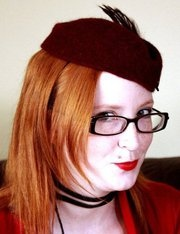
\includegraphics[height=0.25\linewidth]{images/HEPL_spectacles_hat}
%\end{center}
%\end{minipage}

\end{xpsectionbox}

%\vspace{0.5cm}

\xpartbox{Near Duplicate Detection}

\begin{xpsectionbox}{Description}{}

An image data-set may contain many near-duplicate images due to multiple postings of the same photograph rescaled or re-compressed. Such near-duplicates need to be identified and grouped and would be represented by the highest quality image.

\begin{minipage}{0.6\linewidth}

{\vspace*{0.2cm}\noindent\hspace*{0.2cm}{\bf\Titlesize Solution}\newline}{\vspace{-0.75cm}}

\begin{itemize}
	\item Haar wavelet based descriptor: most significant wavelet coefs
	\item real-valued distance measure in $[0,1]$, with 0 = perfect match
	\item low threshold for \emph{near}-duplicate detection
	\item champion selection: highest resolution
\end{itemize}
\end{minipage}
\begin{minipage}{0.5\linewidth}

\begin{center}
%			%\hspace{-5cm}
%			\vspace{-1cm}
			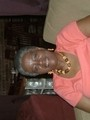
\includegraphics[height=0.25\linewidth]{images/NearDupScaleRot}
			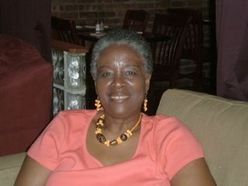
\includegraphics[height=0.25\linewidth]{images/NearDupScale}
\end{center}

\end{minipage}
\end{xpsectionbox}

%\begin{xpsectionbox}{Challenges}{}
%
%\begin{minipage}{0.4\linewidth}
%\begin{itemize}
%	  \item low-quality images
%	  \item various lighting conditions
%	  \item frontal vs. profile faces
%	  \item various skin colors
%	  \item occlusions, facial hair, spectacles, hat, etc.
%\end{itemize}
%\end{minipage}
%\begin{minipage}{0.6\linewidth}
%\begin{center}
%			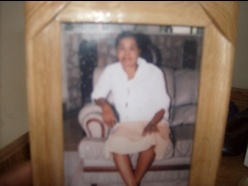
\includegraphics[height=0.25\linewidth]{images/PL_low_quality}
%			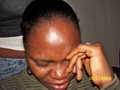
\includegraphics[height=0.25\linewidth]{images/HEPL_occlusion}
%			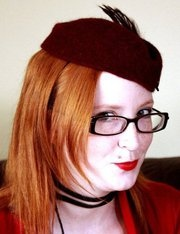
\includegraphics[height=0.25\linewidth]{images/HEPL_spectacles_hat}
%\end{center}
%\end{minipage}
%
%\end{xpsectionbox}
%
%\xpartbox{Solution}
%
%%--------------------------------------------------------------------------------------------------------------------
%\begin{xpsectionbox}{}{}
%
%
%\begin{minipage}{0.5\linewidth}
%\bf{Method:}
%
%\begin{itemize}
%	  \item Haar like features  
%	  \item moving window technique
%	  \item Ada boost classifier cascade
%\end{itemize}
%\begin{center}
%			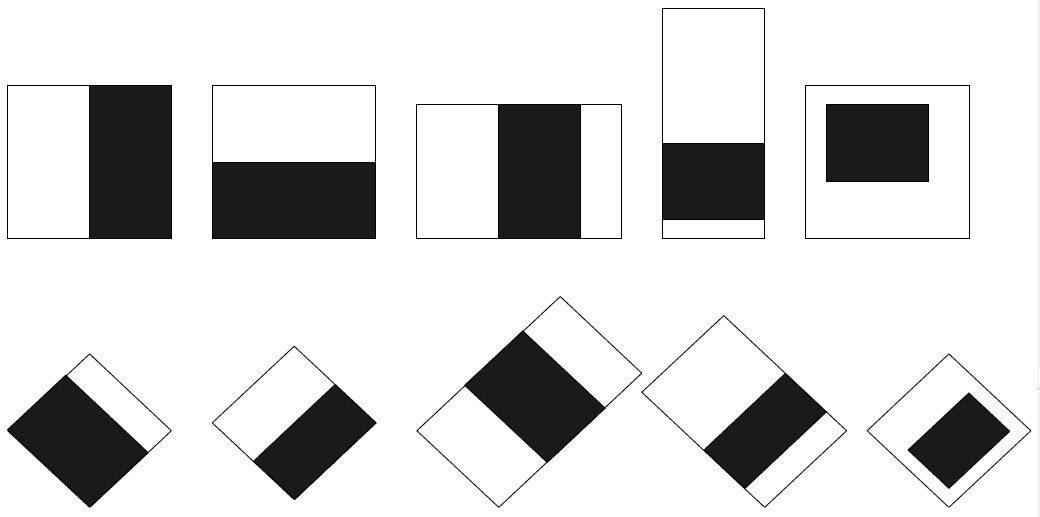
\includegraphics[height=0.25\linewidth]{images/Haar_features}
%\end{center}
%
%\bf{Drawbacks:}
%\begin{itemize}
%	  \item small size faces not detectable
%	  \item lighting/occlusion deteriorates results 
%\end{itemize}
%\begin{center}
%			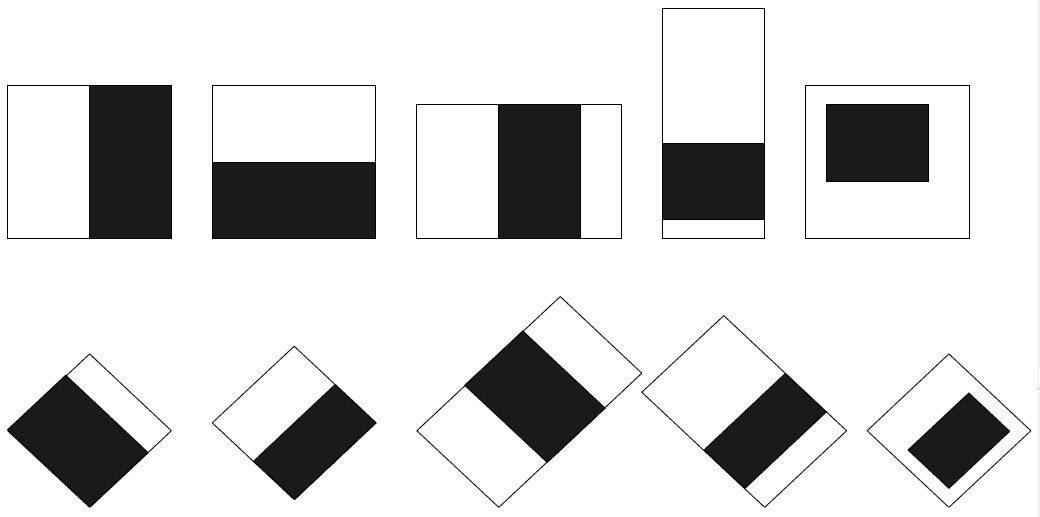
\includegraphics[height=0.25\linewidth]{images/Haar_features}
%\end{center}
%
%\end{minipage}
%\begin{minipage}{0.5\linewidth}
%\bf{Improvements:}
%
%\begin{itemize}
%	  \item color information (skin) 
%	  \item learning color models
%	  \item extended color space + neural network
%\end{itemize}
%\begin{center}
%			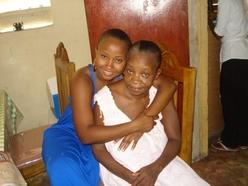
\includegraphics[height=0.2\linewidth]{images/Lena_RGB}
%			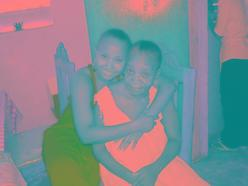
\includegraphics[height=0.2\linewidth]{images/Lena_LAB}
%			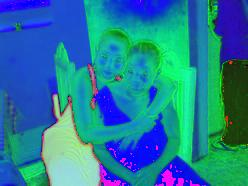
\includegraphics[height=0.2\linewidth]{images/Lena_HSV}
%			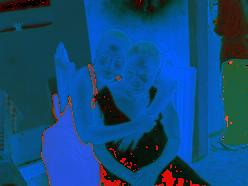
\includegraphics[height=0.2\linewidth]{images/Lena_LUV}
%\end{center}
%\bf{Advantages:}
%\begin{itemize}
%	  \item high precision skin detection(91\%)  
%	  \item skin maps focus the face finding
%	  \item enhance skin region intensities
%\end{itemize}
%\begin{center}
%			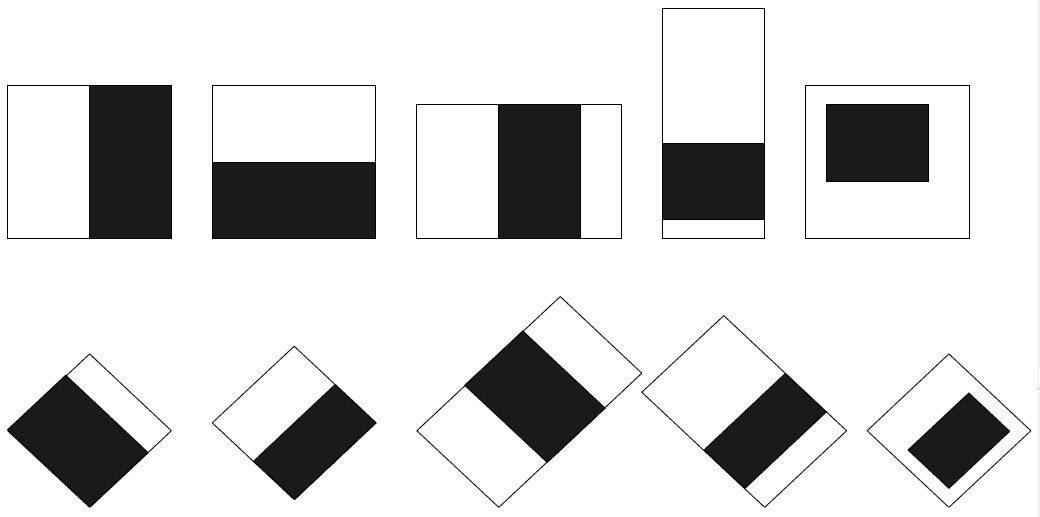
\includegraphics[height=0.2\linewidth]{images/Haar_features}
%\end{center}
%\end{minipage}
%\end{xpsectionbox}

\xpartbox{Experiments}

\begin{xpsectionbox}{}{}
Number of near-duplicates in data-sets % TODO: a table may work better
\begin{itemize}
	\item HEPL: 6K near-dups in 15K images
	\item PL: 4K near-dups in 12K images
\end{itemize}
We have also experimented with generating about 800 near-duplicates from a set of 132 unique images by scaling ($s=0.5, 2$), rotating ($\alpha=\pm\pi/12$) and cropping ($c=0.8, 0.65$). Our near-duplicate detector is most sensitive to rotations and cropping, detecting very few of those, while detecting most of the scaled near-duplicates correctly. This result was rather expected, given the Haar wavelet nature of the detector.
\end{xpsectionbox}

%\vspace{2cm}  
\xpartbox{Face Detection}

\begin{xpsectionbox}{Description}{}

Face detection determines the location and the size of a human face in an arbitrary digital image using:

\begin{minipage}{0.4\linewidth}

\begin{itemize}
	  \item low-level image features (Haar, LBP\footnote{T. Ojala, M. Pietikäinen, and D. Harwood, Performance evaluation of texture measures with classification based on Kullback discrimination of distributions, ICPR, 1994})
	  \item high-level facial landmarks (eye(s), nose, mouth, ear(s), chin, etc.)
	  \item skin color	
\end{itemize}
\end{minipage}
\begin{minipage}{0.6\linewidth}

\begin{center}
%			%\hspace{-5cm}
%			\vspace{-1cm}
			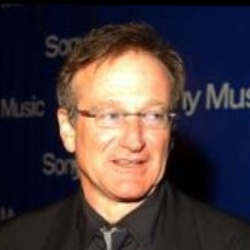
\includegraphics[height=0.25\linewidth]{images/RW_orig}
			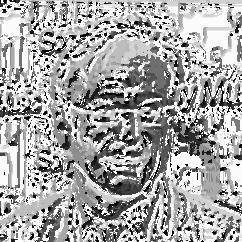
\includegraphics[height=0.25\linewidth]{images/RW_lbp}
			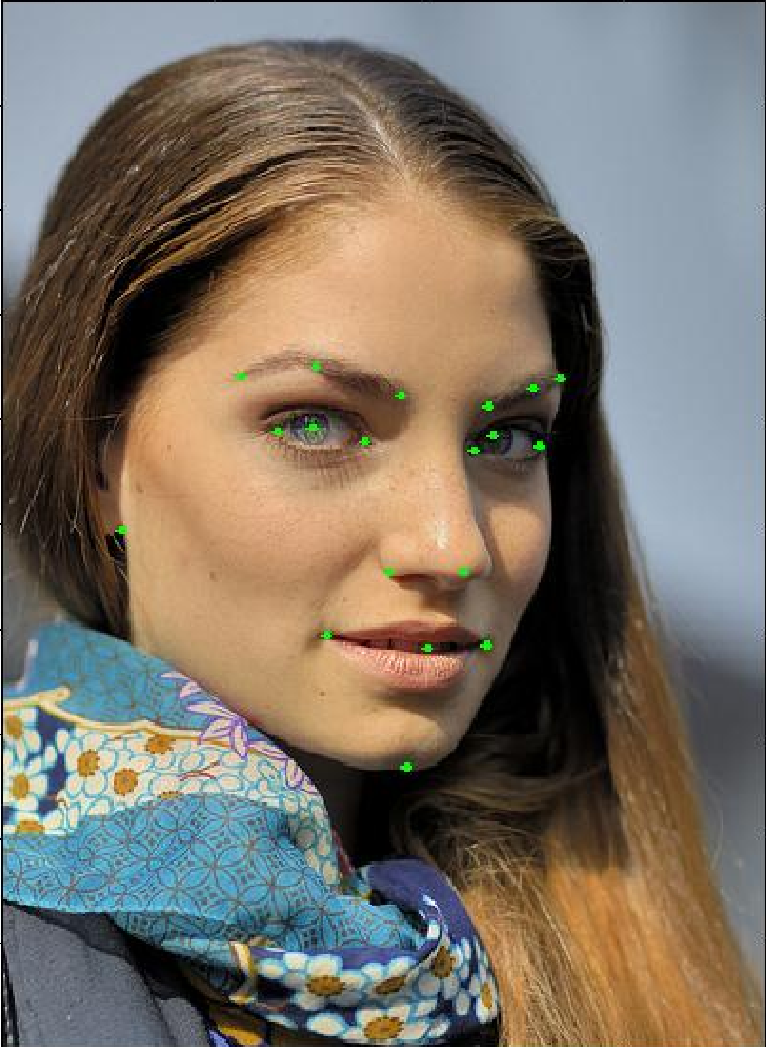
\includegraphics[height=0.25\linewidth]{images/facial_landmarks}
			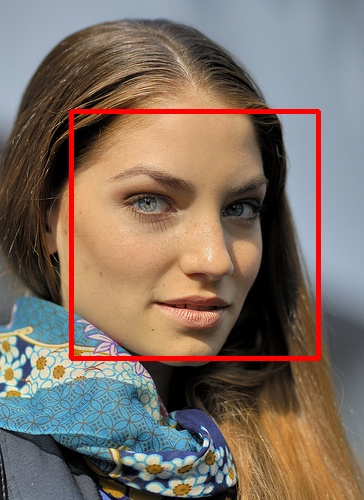
\includegraphics[height=0.25\linewidth]{images/image00168}
\end{center}

\end{minipage}
\end{xpsectionbox}

%\begin{xpsectionbox}{Challenges}{}
%
%\begin{minipage}{0.4\linewidth}
%\begin{itemize}
%	  \item low-quality images
%	  \item various lighting conditions
%	  \item frontal vs. profile faces
%	  \item various skin colors
%	  \item occlusions, facial hair, glasses, hat, etc.
%\end{itemize}
%\end{minipage}
%\begin{minipage}{0.6\linewidth}
%\begin{center}
%			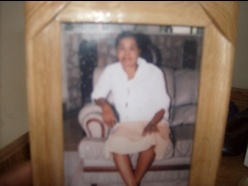
\includegraphics[height=0.25\linewidth]{images/PL_low_quality}
%			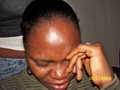
\includegraphics[height=0.25\linewidth]{images/HEPL_occlusion}
%			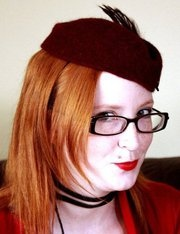
\includegraphics[height=0.25\linewidth]{images/HEPL_spectacles_hat}
%\end{center}
%\end{minipage}
%
%\end{xpsectionbox}

\xpartbox{Solution}

%--------------------------------------------------------------------------------------------------------------------
\begin{xpsectionbox}{}{}


\begin{minipage}{0.5\linewidth}

{\vspace*{0.2cm}\noindent\hspace*{0.2cm}{\bf\Titlesize Method}\newline}{\vspace{-0.75cm}}

\begin{itemize}
	  \item Haar like features  
	  \item moving window technique
	  \item Ada boost classifier cascade (Viola-Jones\footnote{P. Viola and M. Jones, Rapid Object Detection using a Boosted Cascade of Simple Features, CVPR, 2001})
\end{itemize}
\begin{center}
			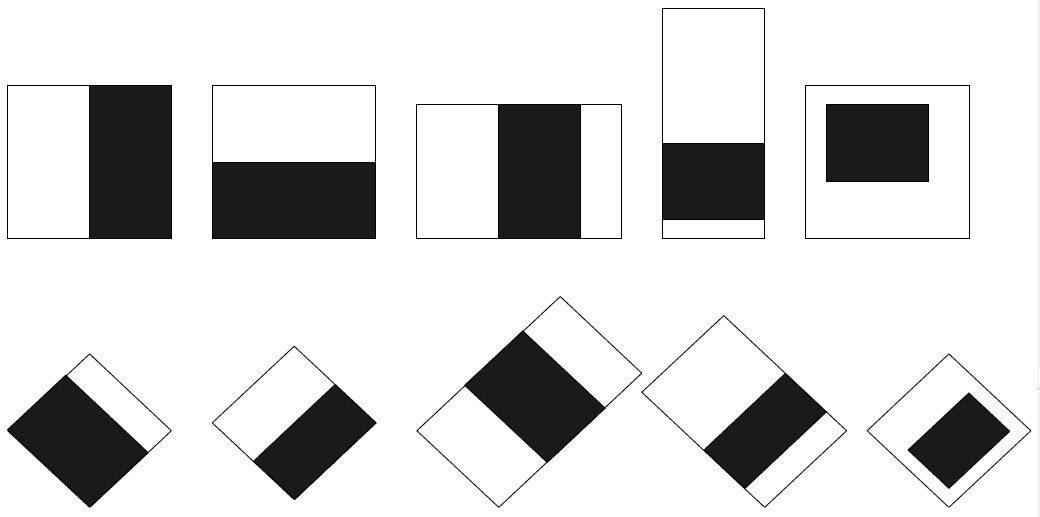
\includegraphics[height=0.25\linewidth]{images/Haar_features}
\end{center}

{\vspace*{0.2cm}\noindent\hspace*{0.2cm}{\bf\Titlesize Drawbacks}\newline}{\vspace{-0.75cm}}

\begin{itemize}
	  \item small size faces not detectable
	  \item lighting/occlusion deteriorates results 
\end{itemize}
\begin{center}
			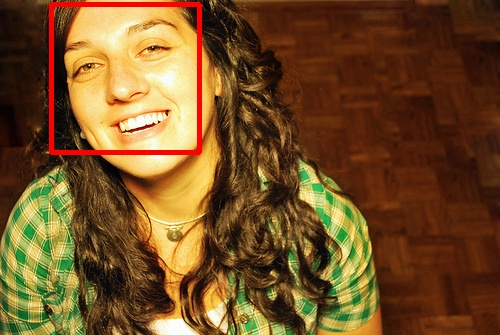
\includegraphics[height=0.2\linewidth]{images/image00613}
			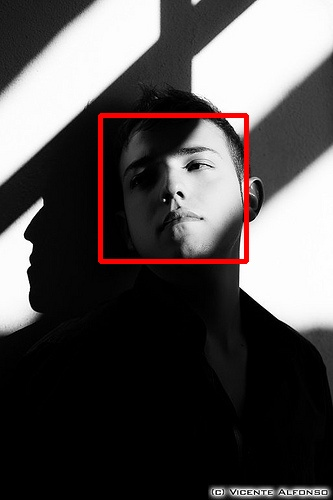
\includegraphics[height=0.2\linewidth]{images/image00571}
			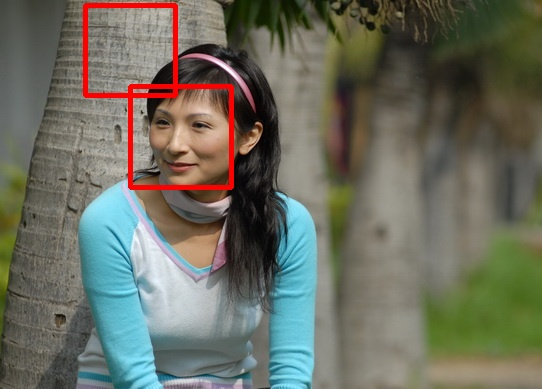
\includegraphics[height=0.2\linewidth]{images/image00210}
\end{center}

\end{minipage}
\begin{minipage}{0.5\linewidth}

\vspace{-2.5cm}
{\vspace*{0.2cm}\noindent\hspace*{0.2cm}{\bf\Titlesize Improvements}\newline}{\vspace{-0.75cm}}

\begin{itemize}
	  \item color information (skin) 
	  \item learning color models
	  \item extended color space + neural network
\end{itemize}
\begin{center}
			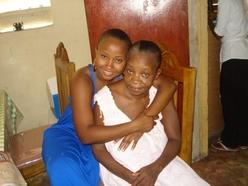
\includegraphics[height=0.16\linewidth]{images/Lena_RGB}
			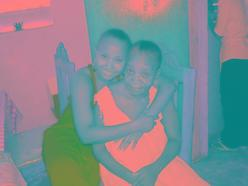
\includegraphics[height=0.16\linewidth]{images/Lena_LAB}
			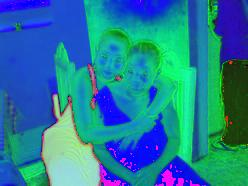
\includegraphics[height=0.16\linewidth]{images/Lena_HSV}
			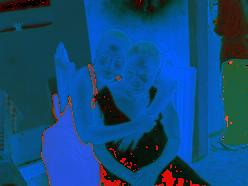
\includegraphics[height=0.16\linewidth]{images/Lena_LUV}
\end{center}

{\vspace*{0.2cm}\noindent\hspace*{0.2cm}{\bf\Titlesize Advantages}\newline}{\vspace{-0.75cm}}

\begin{itemize}
	  \item high precision skin detection(91\%)  
	  \item skin maps focus the face finding
	  \item enhance skin region intensities
\end{itemize}
\begin{center}
			
			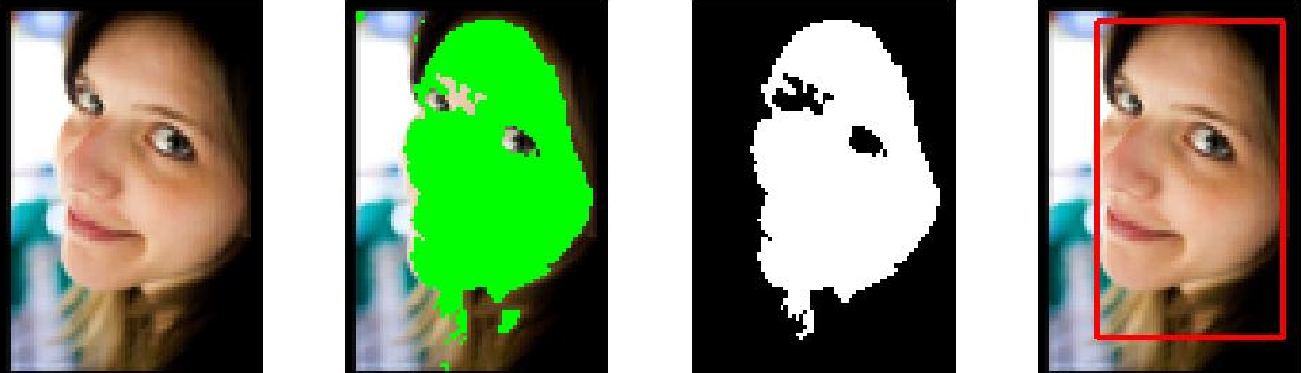
\includegraphics[height=0.2\linewidth]{images/skin_color_demo}
\end{center}
\end{minipage}
\end{xpsectionbox}

\xpartbox{Experiments}

\begin{xpsectionbox}{}{}
With no modifications, Viola-Jones face detector misses about half of the HEPL faces, and about 20\% of the missed ones are typically too small for matching purposes.

Accuracy results of our FaceFinder
\begin{itemize}
	\item HEPL-300: R=75\%, P=83\%, F=79\%
	\item HEPL-4K (noisy): F=53\%
	\item PL-700nd+skin: 46\% Recall boost with 22\% FP rate
\end{itemize}
The major factors hurting the accuracy are: Lighting=5.3\%; Quality=8.8\%; Occlusion=10.8\%; Color=0.6\%; Combination=9.5\%; Small Faces=20.8\%; Other=44.2\%.
\end{xpsectionbox}


%\xpartbox{Evaluation data}
%%--------------------------------------------------------------------------------------------------------------------
%\begin{xpsectionbox}{Data description}{}
%
%\begin{minipage}{0.4\linewidth}
%\begin{itemize}
%		\item $50$ Bangla city names (vocabulary)
%		\item $163$ writers
%	  \item $14,073$ city name samples
%	  \item $7,557$ samples for training (87 writers)
%	  \item $6,516$ samples for test (76 writers)
%	  \item data annotated on word level
%\end{itemize}
%\end{minipage}
%\nolinebreak
%\begin{minipage}{0.6\linewidth}
%		\begin{center}
%			%\hspace{-5cm}
%			\vspace{-1cm}
%			%\includegraphics[height=0.5\linewidth]{images/BanglawordSamples.pdf}\\%
%		\end{center}
%\end{minipage}
%\end{xpsectionbox}
%
%%--------------------------------------------------------------------------------------------------------------------
%
%
%%--------------------------------------------------------------------------------------------------------------------
%%\begin{xpsectionbox}{Network setup}{}
%%\begin{minipage}{0.7\linewidth}
%%\begin{itemize}
%%	  \item fully connected multi-layer perceptron
%%	  \item sigmoid transfer function
%%	  \item error back-propagation
%%	  \item $784-500-10$ topology
%%	  
%%\end{itemize}
%%\end{minipage}
%%\nolinebreak
%%	\begin{minipage}{0.3\linewidth}
%%		\begin{center}
%%			\hspace{-5cm}
%%			\vspace{1.5cm}
%%			\includegraphics[height=0.75\linewidth]{images/mlp.jpg}\\%
%%		\end{center}
%%	\end{minipage}
%%\end{xpsectionbox}
%%--------------------------------------------------------------------------------------------------------------------
%%--------------------------------------------------------------------------------------------------------------------
%%--------------------------------------------------------------------------------------------------------------------
%
%
%
%\xpartbox{Evaluation results}
%
%\begin{xpsectionbox}{Writer independent word recognition}{}
%
%{\bf Model details:}
% 
%\begin{itemize}
%		\item semi-continuous HMMs (ESMERALDA)
%	  \item Bakis topology
%	  \item codebook of $1$k Gaussians with diagonal covariance matrices
%	  \item 20 Baum-Welch training epochs
%\end{itemize}	
%
%\vspace{2cm}
%
%{\bf Recognition results achieved for differently structured writing models:}
%\vspace{1cm}
%
%		\begin{center}	
%    \begin{tabular}{l|r|r|r}
%	Writing Model	&	\multicolumn{2}{c|}{Complexity} &	Rec. Rate \\
%			&	units &	indep. states &	[\%] \\
%	\hline
%	\hline
%	holistic &		50 &	1,645 &	88.0	\\
%	combined characters &	93 &	876 &	88.5	\\
%	pseudo-characters &	52 &	286 &	91.0	\\
%	context-dependent &	293 &	362 (1,714) &	93.1	\\
%	\hline
%	\end{tabular}
%    \end{center}
%    %\caption{Recognition results achieved for differently structured writing models}
%    %\label{tab:results}
%%\end{table}
%
%\vspace{2cm}
%
%{\bf Comments:} 
%\begin{itemize}
%		\item holistic: each word is represented as a single entity
%	  \item combined-characters: modeling basic character, modifiers and combined characters
%	  \item pseudo-characters: modeling just basic character shapes and modifiers
%	  \item context-dependent: modeling pseudo characters and their left and right context
%\end{itemize}	
%\end{xpsectionbox}

%\vspace{1cm}  

\xpartbox{Face Matching}

\begin{xpsectionbox}{Description}{}

Localized face/profile regions  need to be matched against a query face/profile picture, which may come from an existing (and possibly annotated) image, or from a new photograph, that face matcher has not seen before. Hence the face matching method needs to be approximate to accommodate wide variations in the appearance, yet it needs to be fairly exact to eliminate numerous false positive hits.

%\begin{minipage}{0.4\linewidth}
%
%\begin{itemize}
%	  \item low-level image features (Haar, LBP, etc.)
%	  \item high-level facial landmarks (eye(s), nose, mouth, ear(s), chin, etc.)
%	  \item skin color
%\end{itemize}
%\end{minipage}
%\begin{minipage}{0.6\linewidth}
%
%\begin{center}
%%			%\hspace{-5cm}
%%			\vspace{-1cm}
%			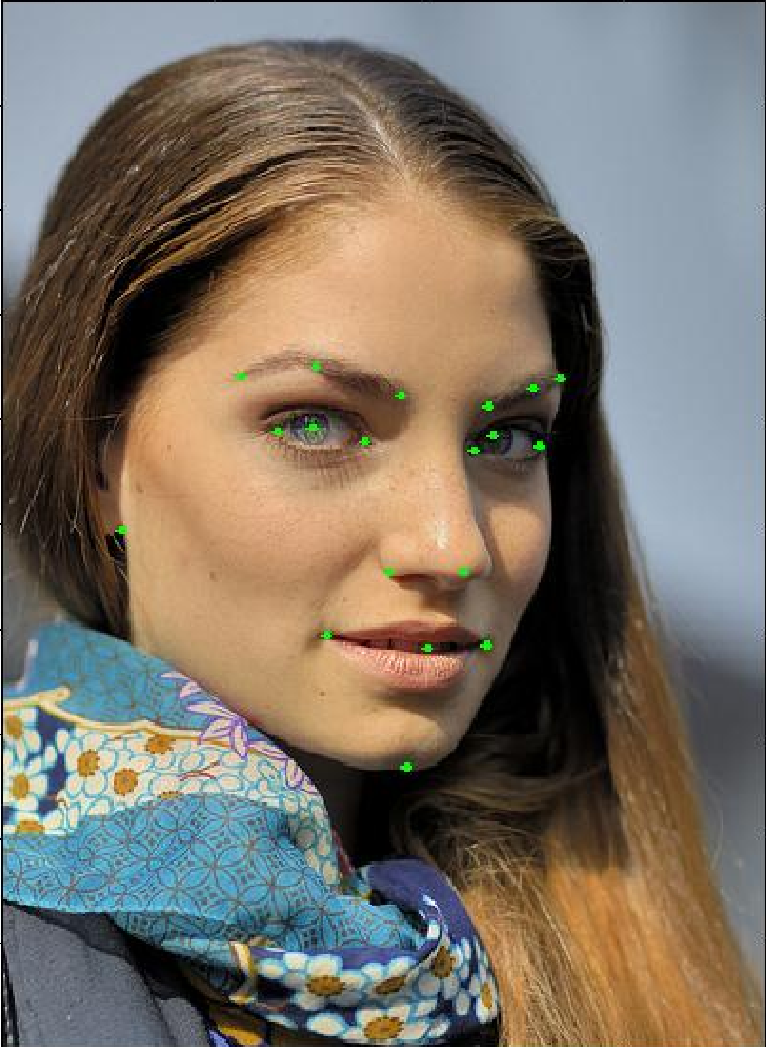
\includegraphics[height=0.25\linewidth]{images/facial_landmarks}
%			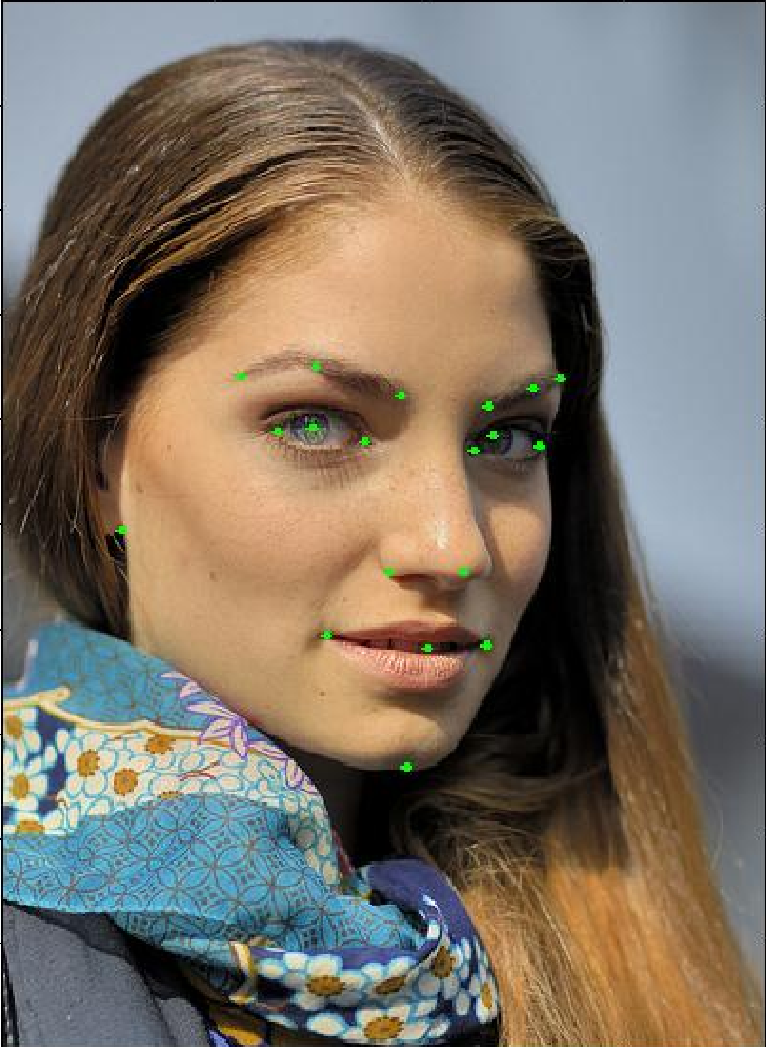
\includegraphics[height=0.25\linewidth]{images/facial_landmarks}
%\end{center}
%
%\end{minipage}
\end{xpsectionbox}

\begin{xpsectionbox}{Challenges}{}

\begin{minipage}{0.4\linewidth}
\begin{itemize}
	  \item local descriptors (Haar, SIFT, SURF, ORB)
	  \item low-quality images
	  \item various lighting conditions
	  \item frontal vs. profile faces
	  \item occlusions, facial hair, spectacles, hat, etc.
\end{itemize}
\end{minipage}
\begin{minipage}{0.6\linewidth}
\begin{center}
			\vspace{-2cm}
			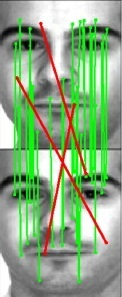
\includegraphics[height=0.45\linewidth]{images/face_match_sift}
\end{center}
\end{minipage}

\end{xpsectionbox}

\xpartbox{Solution}

%--------------------------------------------------------------------------------------------------------------------
\begin{xpsectionbox}{}{}


\begin{minipage}{0.5\linewidth}
Method
\begin{itemize}
	  \item Haar/SIFT/SURF/ORB
	  \item rotation invariant metrics
	  \item ...
\end{itemize}
\begin{center}
			\includegraphics[height=0.25\linewidth]{images/face_sift}
\end{center}

%\bf{Drawbacks:}
%\begin{itemize}
%	  \item small size faces not detectable
%	  \item lighting/occlusion deteriorates results 
%\end{itemize}
%\begin{center}
%			\includegraphics[height=0.25\linewidth]{images/Haar_features}
%\end{center}

\end{minipage}
\begin{minipage}{0.5\linewidth}
Improvements:
\begin{itemize}
	  \item re-ranking based on
	  	\begin{itemize}
	  		\item Borda count
	  		\item weighted Borda count
	  		\item distances
	  	\end{itemize}
	  \item fast indexing (tree structure)
	  \item ...
\end{itemize}
\begin{center}
			%\includegraphics[height=0.2\linewidth]{images/Lena_RGB}
			%\includegraphics[height=0.2\linewidth]{images/Lena_LAB}
			%\includegraphics[height=0.2\linewidth]{images/Lena_HSV}
			%\includegraphics[height=0.2\linewidth]{images/Lena_LUV}
\end{center}
%\bf{Advantages:}
%\begin{itemize}
%	  \item high precision skin detection(91\%)  
%	  \item skin maps focus the face finding
%	  \item enhance skin region intensities
%\end{itemize}
%\begin{center}
%			\includegraphics[height=0.2\linewidth]{images/Haar_features}
%\end{center}
\end{minipage}
\end{xpsectionbox}

\xpartbox{Experiments}

\begin{xpsectionbox}{Results}{}
Our experiments with the annotated HEPL-4K images, and on HEPL-62mod (372 = 62 images with 6 synthetic modifications, e.g. crop, scale and rotate). Accuracy (F-score) figures are reported in the table.

\begin{tabular*}{0.75\textwidth}{@{\extracolsep{\fill}} | c | c | c | c | c | }
  \hline
  dataset & HAAR & SIFT & SURF & ORB \\
  \hline
  HEPL-4K & {\bf0.99} & 0.98 & 0.96 & 0.95 \\
  \hline
  HEPL-62mod  & 0.44  & {\bf0.81}  & 0.52 & 0.56 \\
  \hline
\end{tabular*}

We have also experimented with combining the descriptor match distances by using a generalized geometric mean, and found that a combination of HAAR*ORB*SIFT*SURF produce a better F score (by about 5 percentage points), than either of them. Inclusion of a weak descriptor may hurt the ensemble.
\end{xpsectionbox}

%\xpartbox{Automatic Bangla Recognition}
%
%%--------------------------------------------------------------------------------------------------------------------
%\begin{xpsectionbox}{Motivation}{}
%
%With the availability of electronic tablets at a cost affordable to common Indians, online handwriting recognition for Indian scripts has gained importance.
%
%\begin{minipage}{0.6\linewidth}
%
%\vspace{1cm}
%{\bf Existing problems:}
%
%\begin{itemize}
%	  \item no unconstrained online Indian script recognizer  
%	  \item large symbol set for Bangla
%	  \item no reliable segmentation strategy for Bangla
%\end{itemize}
%
%
%{\bf General solutions:}
%
%\begin{itemize}
%	  \item analytical (segmentation based on pseudo-characters, graphemes), etc. followed by classification   
%	  \item holistic (no segmentation, limited to small vocabulary)
%	  \item HMM based (segmentation and recognition integrated in the model)
%\end{itemize}
%
%{\bf Proposed approach:  Combination of ...}
%
%\begin{itemize}
%	  \item sub-stroke level feature representation
%	  \item HMM based model for cursively written words
%	  \item context dependent sub-word units
%\end{itemize}
%
%\end{minipage}
%\begin{minipage}{0.4\linewidth}
%\begin{center}
%		\vspace{-1cm}
%		\hspace{1cm}
%		\center
%		%\includegraphics[width=0.95\linewidth]{images/input-using-handwriting-recognition.jpg}
%		%\includegraphics[width=0.99\linewidth]{images/tablet.jpg}
%		%\includegraphics[width=0.95\linewidth]{images/hp_tablet.jpg}
%		Wacom Intuos2
%		%\includegraphics[width=0.95\linewidth]{images/Wacom-Intuos2.jpg}
%		\end{center}
%
%\end{minipage}
%
%\end{xpsectionbox}
%%--------------------------------------------------------------------------------------------------------------------
%
%\xpartbox{Preprocessing}
%
%%--------------------------------------------------------------------------------------------------------------------
%\begin{xpsectionbox}{Preprocessing and Sub-Stroke Segmentation}{}
%
%\begin{minipage}{0.5\linewidth}
%
%{\bf Preprocessing:}
%
%\begin{itemize}
%	  \item size normalization (100, original aspect ratio)   
%	  \item smoothing (moving average)
%	  \item re-sampling (distance between two points is $7.0$)
%\end{itemize}
%\end{minipage}
%\begin{minipage}{0.5\linewidth}
%
%
%\vspace{-1.3cm}
%{\bf Stroke segmentation:}
%
%
%\begin{itemize}
%	  \item each stroke is divided in sub-strokes  
%	  \item each sub-stroke with length less than $5$ is discarded
%\end{itemize}
%\end{minipage}
%
%\begin{center}
%		%\vspace{-3cm}
%		%\hspace{1cm}
%		%\center
%		%\includegraphics[width=0.5\linewidth]{images/Aassam-SubStrokes-Numbered.pdf}
%		
%		%\includegraphics[width=0.85\linewidth]{images/unbalanced.pdf}
%\end{center}
%
%{\bf Algorithm:}
%
%\vspace{0.5cm}
%
%\noindent \(P_0, P_1, P_2, \ldots, P_N\) sequence of points from a stroke
%
%\noindent STEP 1: \(i = 0;\) \(j = 1;\)
%
%\noindent STEP 2: Compute \(\theta = \mbox{angle}(P_i,P_j);\)
%
%\noindent STEP 3: {\bf If} \((j < N+1)\)
%
%\hspace{2cm} Compute \(\alpha_j\) = angle \((P_i,P_j);\) %and
%
%\hspace{2cm} \(\beta_j\) = angle \((P_{j-1}, P_j);\)
%
%\hspace{1.2cm} {\bf else}
%
%\hspace{2cm} go to STEP 6
%
%\noindent STEP 4: \hspace{-0.3cm}{\bf If} $(\min\{|\theta-\alpha_j|,360^\circ-|\theta-\alpha_j|\} < 90^\circ \mbox{ and }\min\{|\beta_{j-1}-\beta_j|, 360^\circ-|\beta_{j-1}-\beta_j|\} < 90^\circ)$
%
%\hspace{2cm} \(j = j + 1;\)
%
%\hspace{2cm} GOTO STEP 3
%
%\noindent STEP 5: Segment the stroke at \(P_{j-1}\)
%
%\hspace{1.2cm} \(i = j;\) \(j = j + 1;\)
%
%\hspace{1.2cm} GOTO STEP 2
%
%\noindent STEP 6: STOP
%
%
%\end{xpsectionbox}
%%--------------------------------------------------------------------------------------------------------------------
%
%\xpartbox{Feature Extraction}
%
%%--------------------------------------------------------------------------------------------------------------------
%\begin{xpsectionbox}{Feature Extraction}{}
%
%\begin{minipage}{0.6\linewidth}
%{\bf Steps:}
%
%\begin{itemize}
%	  \item each sub-stroke $S$ is represented by polylines   
%	  \item find six equidistant points \(Q_0,Q_1,\ldots,Q_5\) on $S$
%	  \item calculate the angle $\theta_i$ between x-axis and $Q_{i-1}Q_i$\\ $(i=1,2,\ldots,5;$ $0^\circ \le \theta_i < 360^\circ)$
%		\item normalized gravity center ($\overline{X},\overline{Y})$ of $S$ with respect to\\height ($100$) and width ($W$)
%		\item $l$ is the total length of the sub-stroke $S$
%\end{itemize}
%
%{\bf Result:}
%
%\begin{itemize}
%	  
%		\item 8-dimensional feature vector (\(F=(\theta_1,\ldots,\theta_5,\overline{X},\overline{Y},l)\))
%\end{itemize}
%\end{minipage}
%\begin{minipage}{0.4\linewidth}
%\center
%%\includegraphics[width=0.99\linewidth]{images/sixEquidistantPoints.pdf}
%\end{minipage}
%
%\end{xpsectionbox}
%%--------------------------------------------------------------------------------------------------------------------
%%--------------------------------------------------------------------------------------------------------------------
%
%\xpartbox{Modeling}
%
%\begin{xpsectionbox}{Writing Model}{}
%
%\begin{minipage}{0.6\linewidth}
%
%%\vspace{1cm}
%{\bf Advantages of the modeling:}
%
%\begin{itemize}
%	  \item segmentation/recognition based on HMM 
%	  \item word are constructed from characters
%	  \item complex and robust parameter estimation
%\end{itemize}
%
%\vspace{1cm}
%
%{\bf Challenges in Bangla word modeling:}
%
%\begin{itemize}
%	  \item the notion of basic unit in Bangla is not obvious 
%	  \item basic characters and shape modifiers
%	  \item basic character$+$shape modifiers $=$ new characters
%	  \item characters merged $=$ compound characters
%	  \item potentially huge number of basic modeling units
%\end{itemize}
%
%\vspace{1cm}
%
%{\bf Context-dependent sub-word units for Bangla:}
%
%\begin{itemize}
%	  \item inspired by triphone units from speech recognition
%	  \item Baseline: fully decomposed model (including split up complex modifiers)
%	  \item models include one symbol of left and right context $\Rightarrow$ large number of potential units
%	  \item apply greedy clustering to state-space of intermediate model in order to determine to-be-shared model parameters in purely data-driven manner 
%\end{itemize}
%
%
%\end{minipage}
%\begin{minipage}{0.4\linewidth}
%\begin{center}
%		\vspace{-13cm}
%		\hspace{1cm}
%		\center
%		
%		Basic Bangla characters
%		%\includegraphics[width=0.99\linewidth]{images/BasicCharacter-ICFHR.pdf}
%		
%		
%		\vspace{1cm}
%		Compound Bangla characters
%		%\includegraphics[width=0.99\linewidth]{images/CompoundChar-ICFHR.pdf}
%		\end{center}
%
%\end{minipage}
%
%\vspace{1cm}
%
%\center
%Vowel (left) and consonant (right) modifiers
%%\includegraphics[width=0.99\linewidth]{images/Modifier-ICFHR.pdf}
%
%\end{xpsectionbox}
%--------------------------------------------------------------------------------------------------------------------

%--------------------------------------------------------------------------------------------------------------------

\xpartbox{Conclusion}

\begin{xpsectionbox}{}{}

\begin{minipage}{0.4\linewidth}
\begin{itemize}
	\item important/helpful in disaster scenarios
	\item complementarity between text and images
	\item web interface
		\begin{itemize}
			\item facilitates cooperative work
			\item easy usage
			\item accessibility from remote places
		\end{itemize}
\end{itemize}
\end{minipage}
\begin{minipage}{0.6\linewidth}
\begin{center}
	\includegraphics[height=0.5\linewidth]{images/web_interface}
\end{center}
\end{minipage}

%\begin{minipage}{0.4\linewidth}
%
%\begin{itemize}
%	  \item low-level image features (Haar, LBP, etc.)
%	  \item high-level facial landmarks (eye(s), nose, mouth, ear(s), chin, etc.)
%	  \item skin color
%\end{itemize}
%\end{minipage}
%\begin{minipage}{0.6\linewidth}
%
%\begin{center}
%%			%\hspace{-5cm}
%%			\vspace{-1cm}
%			\includegraphics[height=0.25\linewidth]{images/facial_landmarks}
%			\includegraphics[height=0.25\linewidth]{images/facial_landmarks}
%\end{center}
%
%\end{minipage}
%\end{xpsectionbox}
%
%\begin{xpsectionbox}{Challenges}{}
%
%\begin{minipage}{0.4\linewidth}
%\begin{itemize}
%	  \item low-quality images
%	  \item various lighting conditions
%	  \item frontal vs. profile faces
%	  \item various skin colors
%	  \item occlusions, facial hair, spectacles, hat, etc.
%\end{itemize}
%\end{minipage}
%\begin{minipage}{0.6\linewidth}
%\begin{center}
%			\includegraphics[height=0.25\linewidth]{images/PL_low_quality}
%			\includegraphics[height=0.25\linewidth]{images/HEPL_occlusion}
%			\includegraphics[height=0.25\linewidth]{images/HEPL_spectacles_hat}
%\end{center}
%\end{minipage}

\end{xpsectionbox}





%%
%%%\newpage
%\columnbreak 
%\begin{pcolumn}{0.3}
%%%\input{evaluation}

%%%\xpartbox{Conclusion}

\begin{xpsectionbox}{}{}

\begin{minipage}{0.4\linewidth}
\begin{itemize}
	\item important/helpful in disaster scenarios
	\item complementarity between text and images
	\item web interface
		\begin{itemize}
			\item facilitates cooperative work
			\item easy usage
			\item accessibility from remote places
		\end{itemize}
\end{itemize}
\end{minipage}
\begin{minipage}{0.6\linewidth}
\begin{center}
	\includegraphics[height=0.5\linewidth]{images/web_interface}
\end{center}
\end{minipage}

%\begin{minipage}{0.4\linewidth}
%
%\begin{itemize}
%	  \item low-level image features (Haar, LBP, etc.)
%	  \item high-level facial landmarks (eye(s), nose, mouth, ear(s), chin, etc.)
%	  \item skin color
%\end{itemize}
%\end{minipage}
%\begin{minipage}{0.6\linewidth}
%
%\begin{center}
%%			%\hspace{-5cm}
%%			\vspace{-1cm}
%			\includegraphics[height=0.25\linewidth]{images/facial_landmarks}
%			\includegraphics[height=0.25\linewidth]{images/facial_landmarks}
%\end{center}
%
%\end{minipage}
%\end{xpsectionbox}
%
%\begin{xpsectionbox}{Challenges}{}
%
%\begin{minipage}{0.4\linewidth}
%\begin{itemize}
%	  \item low-quality images
%	  \item various lighting conditions
%	  \item frontal vs. profile faces
%	  \item various skin colors
%	  \item occlusions, facial hair, spectacles, hat, etc.
%\end{itemize}
%\end{minipage}
%\begin{minipage}{0.6\linewidth}
%\begin{center}
%			\includegraphics[height=0.25\linewidth]{images/PL_low_quality}
%			\includegraphics[height=0.25\linewidth]{images/HEPL_occlusion}
%			\includegraphics[height=0.25\linewidth]{images/HEPL_spectacles_hat}
%\end{center}
%\end{minipage}

\end{xpsectionbox}




%\end{pcolumn}

\end{multicols}
\end{poster}
\end{document}


